% We re-run AdaExplore~\citep{adaexplore} and AccelOpt~\citep{accelopt} under the same evaluation harness, the same Claude Opus 4.6 backbone, and the same per-workload \$$10$ optimization-cost budget used by \sys (\autoref{sec:exp-setup}). Both baselines submit through the same compile/correctness/profile gate and are scored against the same vendor reference (\autoref{tab:workloads}). This appendix records what is preserved from each published system and what was necessarily adapted, so that the head-to-head comparison can be reproduced.

% \paragraph{AdaExplore (failure-rule MCTS memory).}
% We reuse the public AdaExplore configuration: failure-rule memory keyed by an extracted failure tag, MCTS-style exploration over an action vocabulary that matches our deoptimization categories, and per-step prompt templates supplied by the released code. The only adaptations are (i) routing all submissions through our harness so that compile/correctness/profile statuses are computed by the same evaluator used for \sys, and (ii) replacing the original budget (a fixed step count) with the cost budget so that all three methods are bounded by the same dollar amount on the same backbone. Failure-rule memory is reset at the start of every workload so that a previous workload's rules cannot leak into the next; this matches the published per-task semantics. We do not modify the search policy, the rule-extraction prompt, or the action vocabulary.

% \paragraph{Filtering out non-kernel wrappers.}
% Across the SM120 AdaExplore runs, several submissions reach the evaluator as wrapper programs: the agent emits a Triton kernel definition, but the surrounding \texttt{ModelNew} catches the kernel-call failure and returns the PyTorch reference. Such submissions can pass correctness and even report a nontrivial speedup, but the measured program is no longer the generated kernel. We confirmed this by rewriting the wrapper's reference-return path into a \texttt{raise}; under the same workload interface, these submissions no longer pass. As a post-hoc audit, we also wired a thin adapter that calls the underlying Conv2d kernels directly with the case-side $(x,w)$ tensors, bypassing the wrapper. This audit recovers two real kernels, but they are much slower than cuDNN (best about $0.41\times$ vs.\ torch and $0.33\times$ vs.\ cuDNN near the end of the run) and require an adapter not produced by AdaExplore's workflow. We therefore mark the SM120 Conv2d number with $\dagger$ in \autoref{tab:appendix-cuda-latencies}: it credits the real audited kernel, not the wrapper's near-parity score. We do not further edit AdaExplore submissions into new task-specific workflows, since such harness-level repair is not an operation organized by the published AdaExplore loop within the shared budget. AccelOpt and \sys do not produce this wrapper pattern in our runs.

% \paragraph{AccelOpt (LLM-summarized memory).}
% For AccelOpt we keep the per-step memory-summary prompt and the iterative refine-with-summary loop from the released system. Memory state is initialized empty per workload, identical to the published per-task semantics. As with AdaExplore, the only adaptations are routing submissions through our evaluator and using the cost budget. We do not introduce skill cards, lineage retrieval, or any \sys-specific memory schema into AccelOpt; its memory remains an LLM-summarized rolling state over the agent's own forward submissions.

% \paragraph{What is shared with \sys.}
% All three methods share the backbone (Claude Opus 4.6), the per-workload cost budget (\$$10$ USD), the evaluator (\texttt{triton.testing.do\_bench}, $100$ reps after $25$ warm-ups), the correctness check (three random seeds), the speedup definition ($T_{\mathrm{ref}}/T_{\mathrm{gen}}$), and the run count ($5$ runs per workload reported as the success-only geometric mean). The vendor reference is the same per platform: cuBLAS for GEMM, cuDNN for Conv2d, FlashInfer for FMHA / Top-K, and FlashInfer or FLA for GDN (\autoref{tab:workloads}). The only thing that varies across methods is the memory representation each one carries between submissions inside a single run.

% \paragraph{What is not preserved.}
% We do not run either baseline beyond \$$10$ in this submission, so we cannot rule out that further dollars would close the gap on individual workloads. We also do not introduce post-training: AdaExplore's failure-rule store and AccelOpt's summarized memory are both held in-context within a single workload's run and discarded between workloads, identical to the published per-task semantics. Per-workload absolute latencies for both baselines are listed alongside \sys in \autoref{tab:appendix-cuda-latencies}.

\section{Baseline Execution and Harness Notes}
\label{sec:appendix-baselines}

We evaluate AdaExplore~\citep{adaexplore} and AccelOpt~\citep{accelopt} in the same external harness used for \sys. This harness standardizes the parts that determine the reported score---input shapes, correctness tests, profiling, vendor references, and cost accounting---while preserving each baseline's own search policy and memory representation. In other words, we do not replace either baseline with a \sys-style memory or planner; each method still decides what to submit using its original in-context state.

All three methods use Claude Opus 4.6 as the online materialization backbone, the per-workload \$$10$ optimization-cost budget, the same compile/correctness/profile gate, and the same vendor reference per platform (\autoref{sec:exp-setup}, \autoref{tab:workload-detail}). We use a dollar budget rather than a fixed submission count because the methods differ in session structure and cache reuse: \sys keeps one prefix-cached chat session per workload, whereas the baselines either restart sessions per submission or use looser caching. The goal is therefore to compare optimization usefulness under the same online cost, not to measure each method's asymptotic ceiling under an unconstrained search horizon.

\paragraph{AdaExplore.}
For AdaExplore, we use the released failure-rule memory, failure-tag extraction, MCTS-style exploration, action vocabulary, and per-step prompt templates. The failure-rule memory is reset at the start of each workload, matching the published per-task setting and preventing rules from one workload from leaking into another. The only harness-level changes are that submissions are routed through our evaluator and budget meter, so that compile status, correctness, latency, and LLM cost are measured consistently with \sys and AccelOpt. We do not modify AdaExplore's search policy, rule-extraction prompt, or memory schema.

\paragraph{Non-kernel wrapper outputs.}
A practical issue arises in some AdaExplore runs: several submissions reach the evaluator as wrapper programs rather than executable generated kernels. The agent emits a Triton kernel definition, but the surrounding \texttt{ModelNew} catches the kernel-call failure and returns the PyTorch reference. Such submissions can pass correctness, and may even appear fast, but the measured program is then the fallback reference path rather than the generated kernel. We verified this by replacing the fallback return path with a \texttt{raise}; under the same workload interface, these submissions no longer pass.

We therefore exclude fallback-wrapper scores from the generated-kernel comparison. To avoid under-crediting AdaExplore, we additionally perform a post-hoc audit for SM120 Conv2d by wiring a thin adapter that directly calls the underlying generated Conv2d kernels with the case-side $(x,w)$ tensors. This audit recovers two real kernels, but they are much slower than cuDNN (best about $0.41\times$ vs.\ torch and $0.33\times$ vs.\ cuDNN near the end of the run), and the adapter itself is not produced by AdaExplore within its workflow. We mark this number with $\dagger$ in \autoref{tab:appendix-cuda-latencies}: it credits the real audited kernel rather than the wrapper's fallback score. We do not otherwise repair AdaExplore submissions or introduce task-specific adapters, since such harness-level repair is outside the published AdaExplore loop and the shared budget.

\paragraph{AccelOpt.}
For AccelOpt, we use the released iterative refine-with-summary loop and its per-step memory-summary prompt. The memory state is initialized empty for each workload, matching the published per-task setting. As with AdaExplore, submissions are routed through our evaluator and budget meter, but the baseline's memory remains an LLM-summarized rolling state over its own forward submissions. We do not introduce SkillCards, lineage retrieval, expert-derived transitions, or any \sys-specific memory schema into AccelOpt.

\paragraph{Shared scoring protocol.}
All three methods share the online backbone, the per-workload cost budget, the evaluator (\texttt{triton.testing.do\_bench} with \texttt{warmup=25} and \texttt{rep=100}, both in milliseconds), the correctness check (three random seeds), the speedup definition ($T_{\mathrm{ref}}/T_{\mathrm{gen}}$), and the run count ($5$ runs per workload, reported as success-only geometric mean). The vendor reference is fixed per platform and workload: cuBLAS for GEMM, cuDNN for Conv2d, FlashInfer for FMHA and Top-K, and FlashInfer or FLA for GDN (\autoref{tab:workload-detail}). Thus, the comparison keeps the model, evaluator, budget, and references fixed; what varies is the optimization memory each method carries between submissions.

\paragraph{Scope of the comparison.}
This comparison evaluates fixed-cost online optimization, not unlimited-horizon search. Search-heavy methods may improve with additional budget, and \sys could also use additional budget for repair and local exploration. Our goal in the main comparison is to ask how useful each memory representation is under the same online materialization cost and validation gate. Per-workload absolute latencies for both baselines are listed alongside \sys in \autoref{tab:appendix-cuda-latencies}.

\paragraph{What an AdaExplore trajectory looks like at the step level.}
\autoref{fig:ada-detail} shows the per-step trajectory for two of the AdaExplore SM120 cases. Panel (a) is GEMM, where $21$ valid kernels are produced over the $\$10$ budget at speedups ranging from $0.57\times$ to $0.88\times$, plus $8$ failed steps; the running-best reaches $0.88\times$ at $\$1.1$ and stays flat afterwards, and most subsequent valid kernels regress below the running-best rather than improve it. Panel (b) is Conv2d, where most steps fail outright ($16$ failed) or emit non-kernel wrappers that compute the right answer through PyTorch ($6$ flagged in the raw trajectory). A thin post-hoc adapter can benchmark two underlying kernels as real Conv2d kernels, reaching about $0.41\times$ near the end of the run, while the remaining wrappers are excluded. The two panels jointly motivate why we report running-best over a wrapper-filtered step set rather than picking the wrapper's reported speedup at face value: the latter would have credited the Conv2d wrappers with about $0.96\times$ on this case.

Green circles denote valid submissions, green diamonds denote adapter-audited kernels, red crosses denote excluded fallback wrappers, and grey triangles denote failed steps. The blue line tracks the best wrapper-filtered speedup, including the audited Conv2d kernels.

\begin{figure*}[h]
\centering
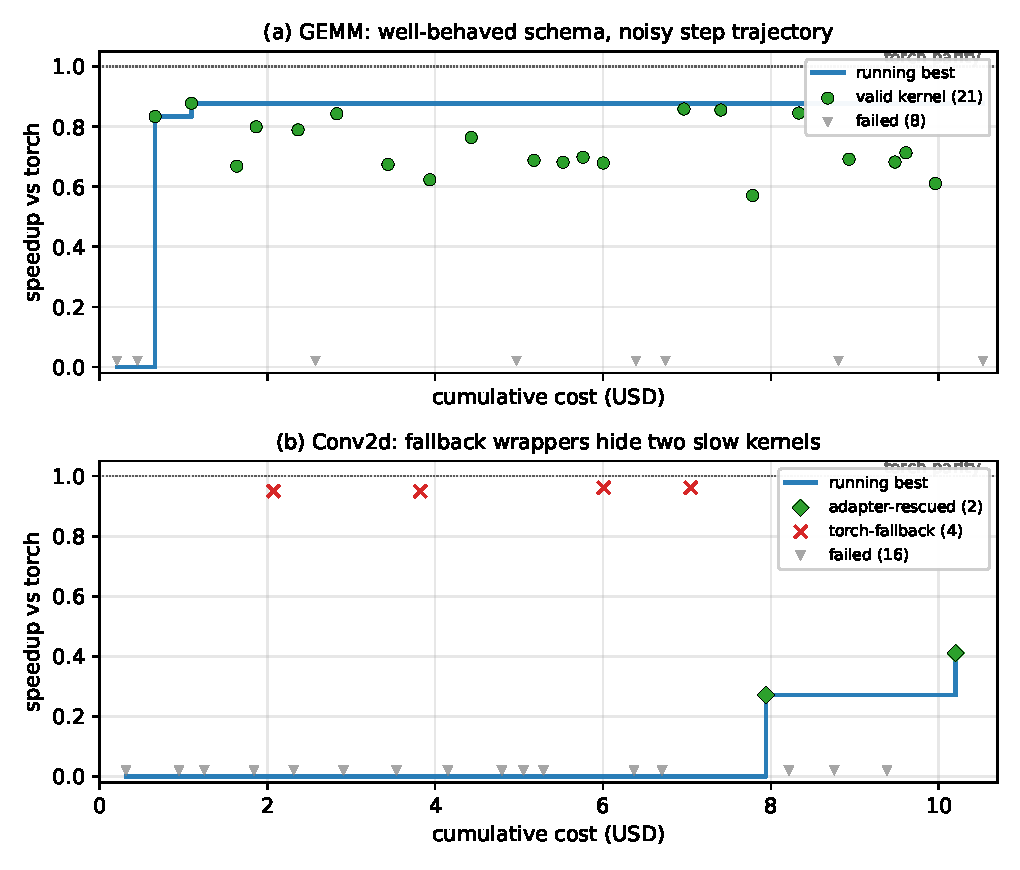
\includegraphics[width=0.78\textwidth]{budget_curve_ada_detail.pdf}
\caption{AdaExplore's SM120 trajectories show repeated regressions on GEMM and frequent failures or fallback wrappers on Conv2d.}
\label{fig:ada-detail}
\end{figure*}
